\documentclass[12pt,letterpaper]{article}
\usepackage{fullpage}
\usepackage[top=2cm, bottom=4.5cm, left=2.5cm, right=2.5cm]{geometry}
\usepackage{amsmath,amsthm,amsfonts,amssymb,amscd}
\usepackage{lastpage}
\usepackage{enumerate}
\usepackage{fancyhdr}
\usepackage{mathrsfs}
\usepackage{xcolor}
\usepackage{graphicx}
\usepackage{listings}
\usepackage{hyperref}

\hypersetup{%
  colorlinks=true,
  linkcolor=blue,
  linkbordercolor={0 0 1}
}
 
\renewcommand\lstlistingname{Algorithm}
\renewcommand\lstlistlistingname{Algorithms}
\def\lstlistingautorefname{Alg.}

\lstdefinestyle{Python}{
    language        = Python,
    frame           = lines, 
    basicstyle      = \footnotesize,
    keywordstyle    = \color{blue},
    stringstyle     = \color{green},
    commentstyle    = \color{red}\ttfamily
}

\setlength{\parindent}{0.0in}
\setlength{\parskip}{0.05in}

% Edit these as appropriate
\newcommand\course{APL 452}
\newcommand\hwnumber{1}                  % <-- homework number
\newcommand\NetIDa{2019ME10770}           % <-- NetID of person #1
\newcommand\NetIDb{Aditya Shankar Garg}           % <-- NetID of person #2 (Comment this line out for problem sets)

\pagestyle{fancyplain}
\headheight 35pt
\lhead{\NetIDa}
\lhead{\NetIDa\\\NetIDb}                 % <-- Comment this line out for problem sets (make sure you are person #1)
\chead{\textbf{\Large Homework \hwnumber}}
\rhead{\course \\ \today}
\lfoot{}
\cfoot{}
\rfoot{\small\thepage}
\headsep 1.5em

\begin{document}

\section*{Problem 2}


\begin{enumerate}
  \item
  \textbf{derive the three step adam-bashforth method's explicit scheme :}
   \newline
   \newline
   we need to interpolate the polynomial $f(t, y(t))$ and then integrate the interpolated polynomial. for this question $s = 3$ hence we will consider a interpolating polynomial of order = 2 passing through $(t_{n-2}, f_{n-2})$, $(t_{n-1}, f_{n-1})$, $(t_{n}, f_{n})$
   \[P_3(\tau) = f_{n-2}L_{n-2}(\tau)+f_{n-1}L_{n-1}(\tau)+f_{n}L_{n}(\tau)\]
   we need to find the $L_i$'s using the following relations : 
   \begin{itemize}
       \item $L_{n-2} = \frac{(\tau - t_{n-1}) (\tau - t_{n})}{(t_{n-2}-t_{n-1})(t_{n-2}-t_{n})} = \frac{1}{2h^2}(\tau - t_{n-1}) (\tau - t_{n})$
       \item $L_{n-1} = \frac{(\tau - t_{n}) (\tau - t_{n-2})}{(t_{n-1}-t_{n-2})(t_{n-1}-t_{n})} = \frac{-1}{h^2}(\tau - t_{n}) (\tau - t_{n-2})$
       \item $L_{n} = \frac{(\tau - t_{n-2}) (\tau - t_{n-1})}{(t_{n}-t_{n-1})(t_{n}-t_{n-2})} = \frac{1}{2h^2}(\tau - t_{n-1}) (\tau - t_{n-2})$
   \end{itemize}
   integrating the expression $y_{n+1} = y_n + \int P_3(\tau) d\tau$ ; which can be written as the following: 
   \[y_{n+3} = y_n + f_{n-2}\int_{t_{n+1}}^{t_n} L_{n-2}(\tau)d\tau + f_{n-1}\int_{t_{n+1}}^{t_n} L_{n-1}(\tau)d\tau + f_{n}\int_{t_{n+1}}^{t_n} L_{n}(\tau)d\tau\]
   
   we need to substitute the variable $\tau$ by a new variable $u = \frac{\tau - t_n}{h} $ such that $0\leq u\leq 1$
   \begin{itemize}
       \item $L_{n-2} = \frac{u(u+1)}{2}$
       \item $L_{n-1} = -u(u+2)$
       \item $L_{n} = \frac{(u+1)(u+2)}{2}$
   \end{itemize}
   
   on integrating we can obtain the following values for all the integrating terms on the right hand side:
   \begin{itemize}
       \item $\int_{t_{n+1}}^{t_n} L_{n-2}(\tau)d\tau =  \frac{h}{2} \int_{0}^{1}\frac{u(u+1)}{2} du = \frac{5}{12}h$
       \item $\int_{t_{n+1}}^{t_n} L_{n-1}(\tau)d\tau =  -h \int_{0}^{1} u(u+2) du = \frac{-4}{3}h$
       \item $\int_{t_{n+1}}^{t_n} L_{n}(\tau)d\tau =  \frac{h}{2} \int_{0}^{1}\frac{(u+2)(u+1)}{2} du= \frac{23}{12}h$
   \end{itemize}
   
   hence we have the update rule for the three step method given by the following relation : 
   \[y_{n+3} = y_n + \frac{h}{12}\left( 5 f_{n-2} - 16 f_{n-1} + 23 f_n\right)\]
  \item
    \textbf{find the order of convergence of the three-eight scheme given in the problem two part (b):}
    \newline
    \newline
    \[y_{n+3} - y_n = h\left(\frac{3}{8} f_{n+3} + \frac{9}{8} f_{n+2} +\frac{9}{8} f_{n+1}+\frac{3}{8} f_{n}\right)\]
    
    the characteristic polynomial for the method is given by : 
    \newline
    \newline 
    $\rho(w) = w^3 - 1$ hence the coefficients are $\alpha_0 = -1$, $\alpha_3 = 1$; the normalising constants $\beta_i$'s are as follows : $\beta_0 = \frac{3}{8}$, $\beta_1 = \frac{9}{8}$, $\beta_2 = \frac{9}{8}$, $\beta_3 = \frac{3}{8}$
    \newline
    \newline
    the order of the method is equal to 4 as $c_0 = c_1 = c_2 = c_3 = c_4 =0$ and $c_5 \not= 0$. we have assumed that the method converges but it can also be shown here as for convergence we need consistence and zero stability which are guaranteed to us using $c_0$ and $c_1$ and the fact that the characteristic polynomial has no roots greater than one and the multiplicity of the root equal to one is also one.
\begin{center}
    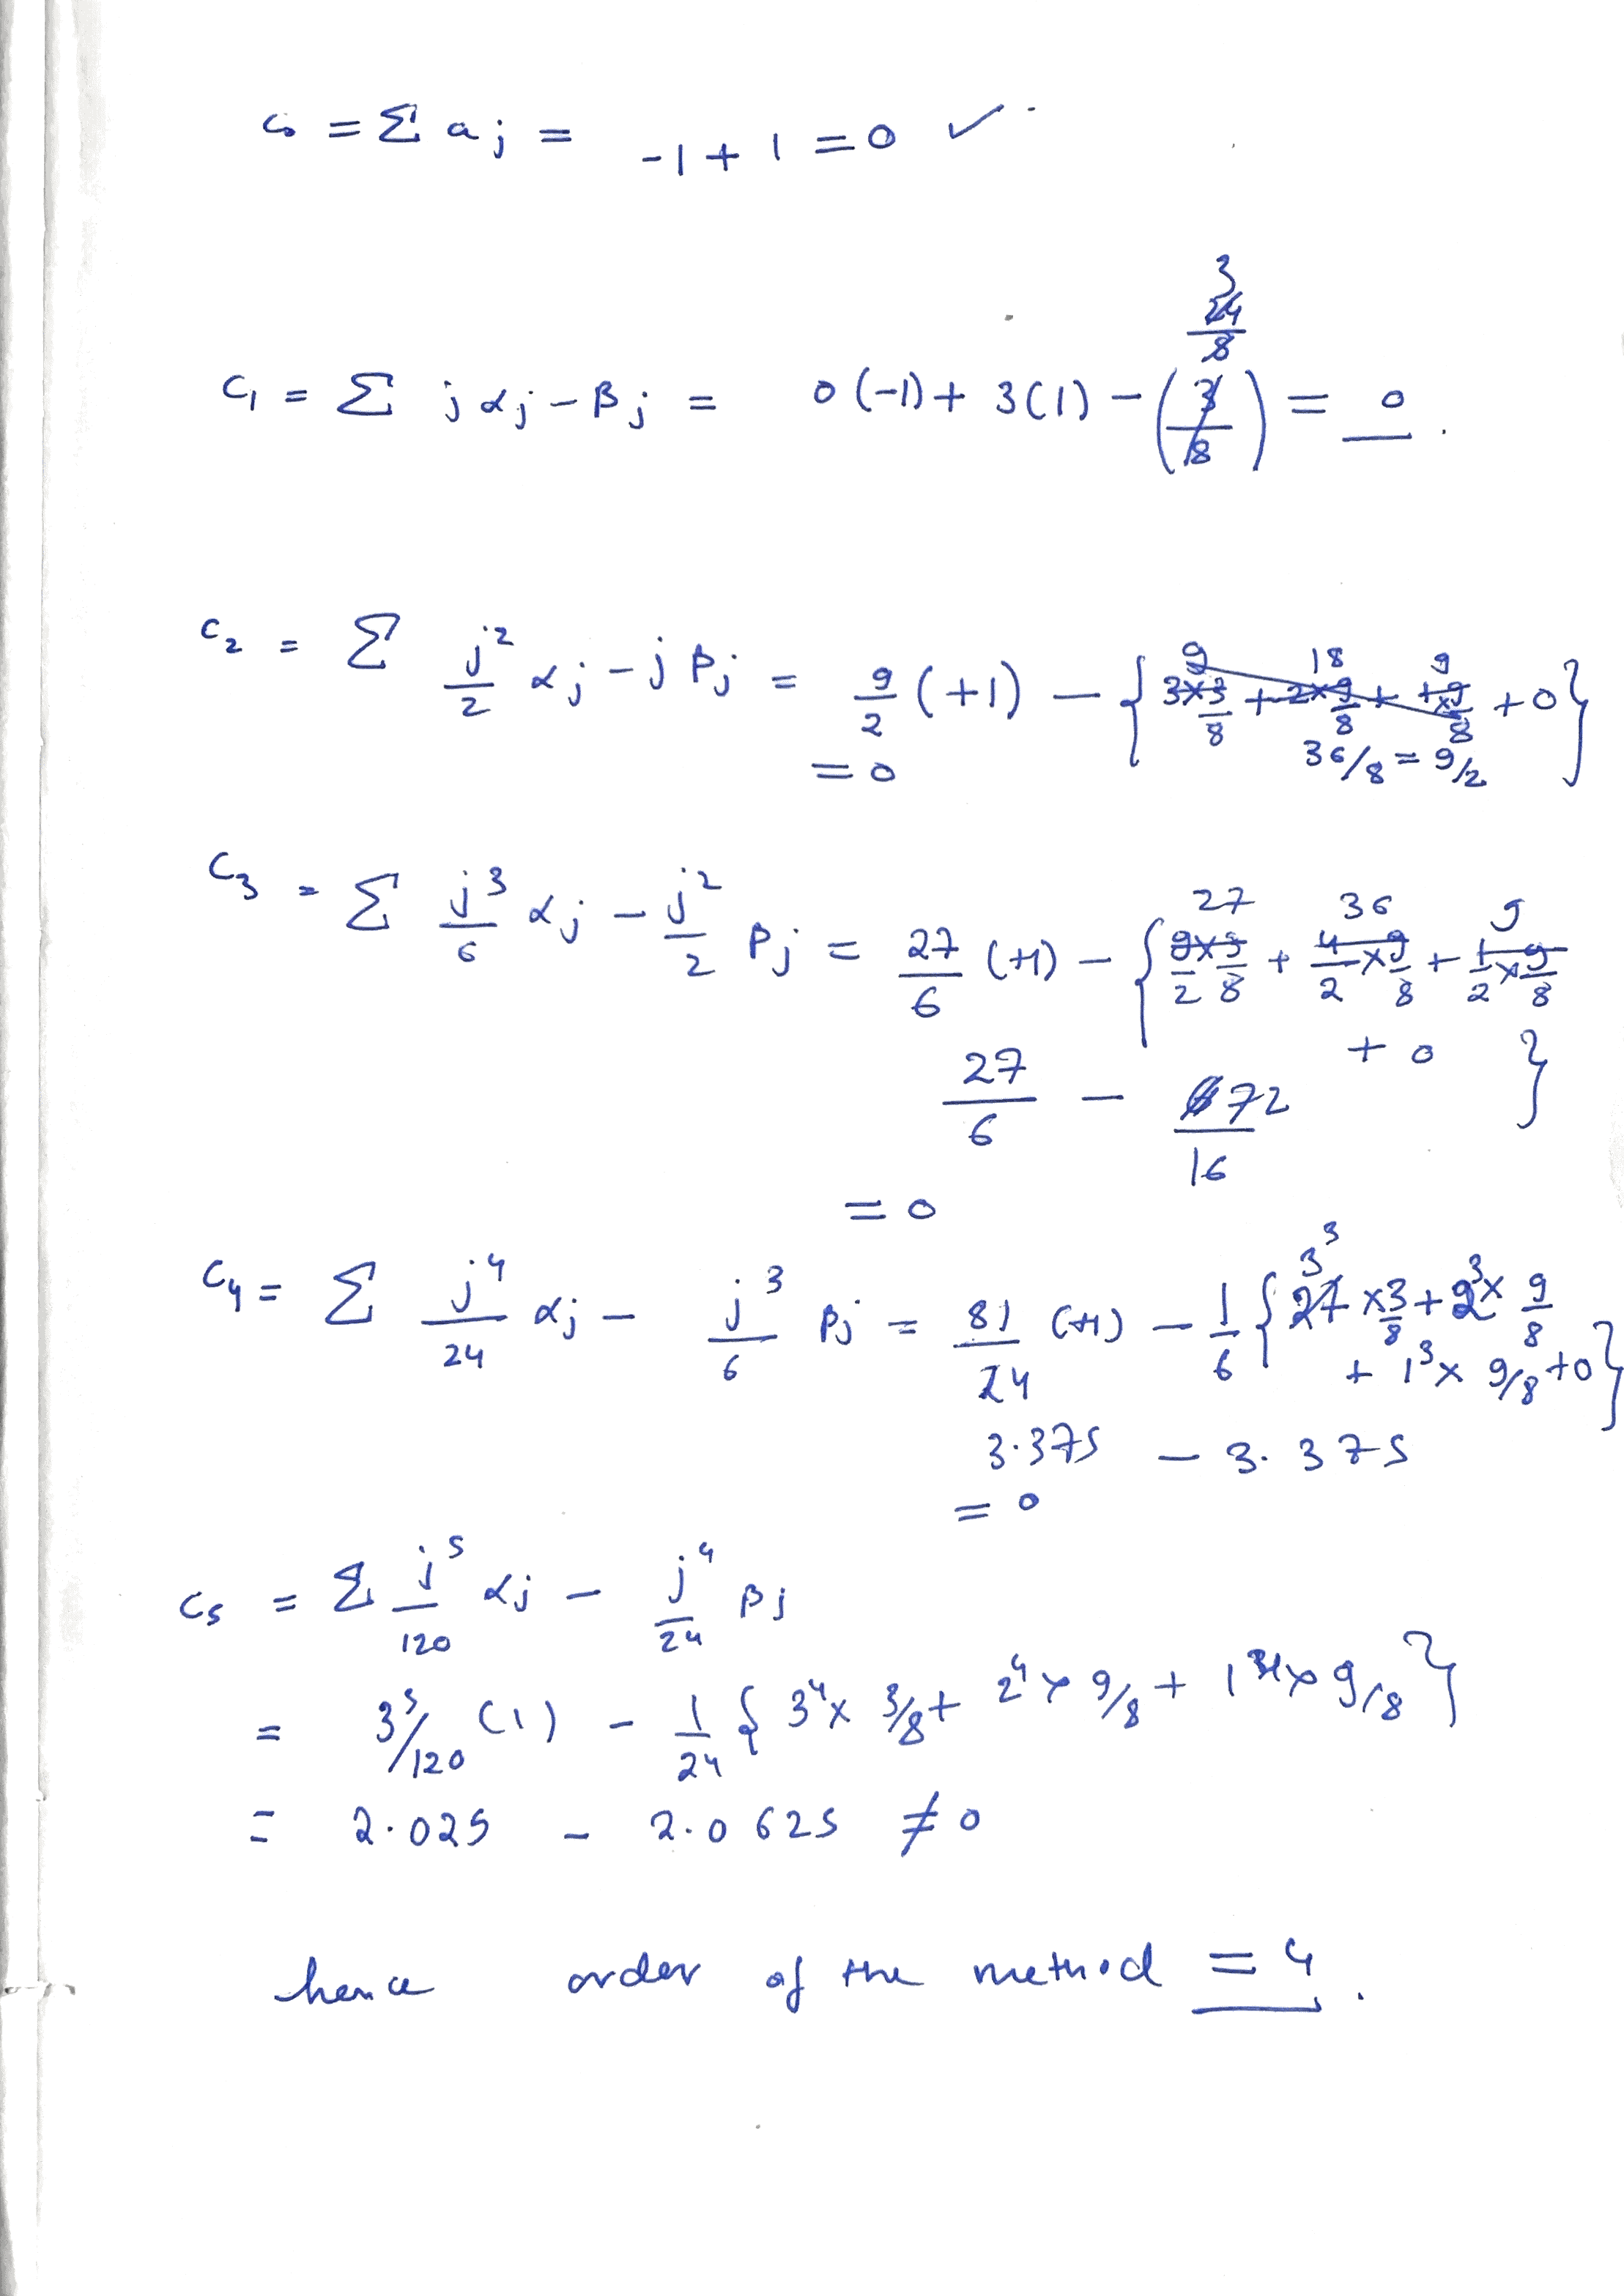
\includegraphics[scale=0.2]{file_1.png}
\end{center}

\end{enumerate}




\end{document}
